
\chapter{Desenvolvimento dos protótipos}
% Label para referenciar
\label{desenvolvimento-prototipos}

% Diminuir espaçamento entre título e texto
\vspace{-1.9cm}

% Texto do capítulo

  Este capítulo apresenta o cenário proposto para o estudo de caso, bem
  como o desenvolvimento dos protótipos com suas fases de implementação, iniciando
  pela elicitação dos requisitos seguindo a abordagem \ac{REST}.
  
  Como serão desenvolvidos dois protótipos com o objetivo de compará-los, iniciaremos o desenvolvimento com o \textit{framework} Django, e por fim, faremos o desenvolvimento
  com o ambiente Node.Js e \textit{framework} Express.Js, formando assim a aplicação proposta.
  
\section{O escopo do projeto}
\label{escopo-projeto}

  Com base nos aspectos abordados ao longo deste trabalho, 
  esta seção visa apresentar o desenvolvimento de um \textit{Web Service} seguindo os padrões \ac{REST} e a utilização 
  de um banco de dados relacional Postgres para a persistência dos dados.  
  Tal serviço possuirá métodos que serão consumidos por dispositivos clientes.

\subsection{Levantamento Requisitos}
\label{levantamento-requisitos}

  Utilizaremos o mesmo exemplo citado por \citeonline{Pereira:2013} pois é de fácil compreensão
  e entendimento de uma simples aplicação. Em seu livro o autor para ensinar o \textit{framework}
  Express.Js e Node.Js cria uma agenda de contatos integrando-o com um Web \textit{chat} funcionando em tempo-real.
  
  A aplicação do autor possui requisitos funcionais bastante objetivos tais como: O usuário cria, edita ou exclui um contato; 
  o usuário realiza \textit{login} informando nome e e-mail; conectar ou desconectar no chat; poder enviar e receber mensagens no chat somente
  dos contatos \textit{online}
  
  Ao investigar o primeiro requisito -(criar, editar ou excluir um contato)- foi possível encaixa-lo neste trabalho pois um serviço em
  REST encaixa perfeitamente nesta necessidade. Como este trabalho não possui o mesmo foco do aplicativo utilizado por \citeonline{Pereira:2013}
  e sim comparar desempenho das aplicações simplificamos o desenvolvimento para cumprir o objetivo deste trabalho.

\subsubsection{Elicitação de requisitos}

  Sendo assim, é possível destacar os seguintes requisitos candidatos:

  \begin{compactitem}
    \item[a)] A \ac{API} \ac{REST} deverá ter um recurso chamado Pessoas.
    \item[b)] A \ac{API} \ac{REST} deverá prover estratégias para manipular as ações de CRUD de uma pessoa(s)
    \item[c)] A \ac{API} \ac{REST} deverá ter um recurso chamado Contatos.
    \item[d)] A \ac{API} \ac{REST} deverá prover estratégias para manipular as ações de CRUD de um contato(s)
  \end{compactitem}
  
\subsubsection{Análise dos requisitos}
  
  Perante os requisitos elicitados verificou-se que o objetivo essencial de uma pessoa, candidato a usuário
  do sistema, é controlar os próprios contatos.
  O principal requisito destacado na análise é registrar estes contatos. Para atender o requisito
  propõem-se a utilização de uma \ac{API} \ac{REST}, para fornecer os \ac{CRUD} de cada recurso
  como na Tabela \ref{tab:api-descricao-contato}.
 
  
  \begin{table}[H]
    \centering
    \footnotesize
    \vspace{0.5cm}
    % Alterar espaçamentos antes e depois do caption
    \setlength{\abovecaptionskip}{0pt}
    \setlength{\belowcaptionskip}{0pt}
    % Caption
    \caption[Descrição da API de contatos]{Descrição da API de contatos}
    \label{tab:api-descricao-contato}
    % Conteúdo da tabela
    \begin{tabular}{c|c|c|p{8cm}}
      \hline \hline
      Metódo  &	Parâmetro &	Recurso &	Descrição \\
      \hline \hline
      GET	& -	& contatos	& Retorna a lista de contatos 
					  cadastrados no banco de dados \\
      \hline \hline
    \end{tabular}
    % Fonte
    \captionfont{\small{\textbf{\\Fonte: Autor}}}
  \end{table}
  
\subsubsection{Tecnologias Utilizadas}


  Aplicativo comparativo Django
    
    \begin{compactitem}
      \item[a)] Python – Linguagem de programação Orientada a Objetos usada na comparação de aplicativos deste trabalho;
      \item[b)] Postgres – Banco de dados relacional
      \item[c)] Django/django-rest-framework – \textit{Framework} Django para aplicações web e o pacote django-rest-framework
      para facilitar o desenvolvimento.
    \end{compactitem}
    
  Aplicativo Node.JS
  
    \begin{compactitem}
      \item[a)] Node.Js – Ambiente de Programação \textit{Backend} para apresentação deste trabalho
      \item[b)] Postgres – Banco de dados relacional
      \item[c)] Express – \textit{Framework} para aplicações web
    \end{compactitem}
 
\subsubsection{Mapeamento de dados}

  De acordo com os requisitos elicitados foi construído o diagrama de entidade e relacionamento para melhor
  documentar estes requisitos.
  
  \begin{figure}[H]
    % Alterar espaçamentos antes e depois do caption
    \setlength{\abovecaptionskip}{0pt}
    \setlength{\belowcaptionskip}{0pt}
    % Caption
    \caption[Diagrama de entidade e relacionamentos]{Diagrama de entidade e relacionamentos}
    \centering
    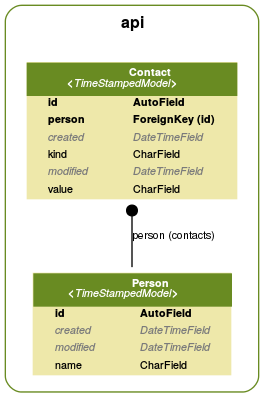
\includegraphics[width=.55\textwidth]{imagem/der.png}
    % Caption centralizada
    \captionsetup{justification=centering}
    \captionfont{\small{\textbf{\\Fonte: Autor}}}	
    \label{fig:der}
  \end{figure}

  Conforme a Figura \ref{fig:der}, os protótipos possui as seguintes tabelas: \textit{Person} e \textit{Contact},
  que fazem o registro de pessoas e contatos, respectivamente, e possui os atributos (campos) necessários
  para armazenar os registros da API no banco de dados. Na entidade de \textit{person}, temos o identificador
  "id" como chave primária, única e auto-incremento, "created" e "modified" como campos de data e o campo
  "nome" para identificar o nome da pessoa. Na tabela de \textit{contact} temos um identificador "id" único e auto-incremento,
  "created" e "modified" como campos de data, "kind" com caracter para saber o tipo do contato e "value" para 
  saber o valor do tipo do contato. A tabela \textit{contact} possui um relacionamento com a tabela \textit{person},
  com a cardinalidade de muitos para um.

  
\section{Aplicação em Django}
\label{desenvolvimento-django}

  Neste capítulo apresenta o desenvolvimento de uma aplicação Django com o pacote Django Rest Framework para que o 
  leitor tenha conhecimento geral sobre o processo de desenvolvimento com este \textit{framework}. 
  
  
\subsection{Instalação Base}

  Para iniciar o desenvolvimento com o \textit{framework} Django é necessário ter instalado no sistema operacional
  (este protótipo foi desenvolvido em Linux) as seguintes bibliotecas: python-pip; python-virtualenv; python-dev;
  libpq-dev.  O python-pip é utilizado para instalar os pacotes do repositório de pacotes do python conhecido como
  PyPI \footnote{The Python Package Index. Disponível em https://pypi.python.org/pypi}. O python-virtualenv é utilizado
  para isolar em um ambiente virtual as bibliotecas instaladas e utilizadas na aplicação para que não corrompa as bibliotecas
  do sistema operacional. O python-dev é um conjunto de ferramentas para o desenvolvimento com a linguagem python e a libpq-dev
  é a biblioteca resposável por compilar e comunicar a aplicação com o \textit{backend} do banco de dados Postgres.
  
  Após instalar essas bibliotecas no sistema operacional, deve seguir as etapas abaixo em ordem.
  
  \begin{compactitem}
    \item[1)] Criar o ambiente virtual;
    \item[2)] Instalar o \textit{framework} Django e o pacote \textit{Django Rest Framework};
    \item[3)] Criar o esqueleto ou estrutura de diretórios da aplicação.
  \end{compactitem}
  
  Para o item 1, execute o comando \textit{virtualenv django\_rest}. Em seguida é necessário ativar este ambiente com o comando
  \textit{source django\_rest\/bin\/activate}. Após a ativação do ambiente prosseguimos para segunda etapa executando o comando
  \textit{ pip install django djangorestframework}
  
  \textbf{****PRECISA FALAR DA HISTORIA DO DJANGO???? *****}
  
  O Django Rest Framework, como descrito em seu site \footnote{Disponível em http://www.django-rest-framework.org/} é uma poderosa
  e flexível caixa de ferramentas para construir API\'s em aplicações Web. Dente suas facilidades pode-se destacar: navegação na API através
  de páginas HTML, politicas de autenticação, serializar os objetos do banco de dados, funções e classes base para prover os recursos
  de uma API e suas respectivas funcionalidades, uma extensa documentação e suporte pela comunidade.
  
  Após a visão geral do pacote, executamos a última etapa para criar a estrutura de diretórios. Para isto use o comando
  \textit{django-admin.py startproject --template https:\/\/github.com\/lucassimon\/django-project-template\/zipball\/master --extension py,md django\_rest}.
  
  Com este comando ira ser criado toda a estrutura necessária para a aplicação faltando poucas alterações e configurações.
  
\subsection{Configurações}

  Entre no diretório criado e faça a instalação dos demais pacotes necessários com o comando \textit{pip install -r requirements\/dev.txt}.
  Em seguida edite o arquivo \textit{settings.py} localizado dentro do diretório \textit{infra\_confs\/} e altere a configuração
  do nome do banco de dados na linha \textit{DATABASE\_URL}.
  
  Altere o arquivo \textit{base.py} dentro do diretório \textit{django\_rest\/settings\/} inserindo na configuração \textit{INSTALLED\_APPS}
  o texto \textit{'rest\_framework'}. Neste mesmo arquivo é necessário setar uma configuração do pacote Django Rest Framework
  com o objetivo de liberar a permissão de acesso para todas os recursos providos no módulo \textit{api}.
  
  \begin{algorithm}[H]
  \KwData{this text}
  \KwResult{how to write algorithm with \LaTeX2e }
  REST\_FRAMEWORK = {
       'DEFAULT\_PERMISSION\_CLASSES': [
          \'rest\_framework.permissions.AllowAny\'
       ]
  }
  \caption{How to write algorithms}
  \end{algorithm}
  
  Para finalizar as configurações executamos o comando \textit{python manage.py syncdb --migrate --settings=django\_rest.settings.dev}
  para sincronizar as configurações com o banco de dados criado.
  
  

\subsection{Desenvolvimento}

  Abaixo segue a metodologia e processos utilizados no desenvolvimento da API em Django.
  
  Para iniciar o desenvolvimento do protótipo é criado o módulo \textit{api}, como descrito anteriormente,
  para isto execute o comando \textit{python manage.py startapp --template https://github.com/lucassimon/django-app-template/zipball/master api}
  
  Através deste comando é criado um diretório de nome \textit{api} contendo os principais arquivos utilizados no decorrer deste protótipo.

\subsubsection{Modelos}

  Primeiro, precisa escrever o modelos através das classes \textit{Person} e \textit{Contacts}. Estas classes irão representar o diagrama
  de entidade e relacionamentos da figura \ref{fig:der}. Na classe \textit{Person} foi definido a coluna \textit{name} como um campo 
  do tipo \textit{char} e 255 caracteres.
  
  \textbf{*** AQUI ROLA DE COLAR CÒDIGO OU FIGURA???? *** }
  
  Na classe model \textit{Contact} temos o atributo prson como chave estrangeira da classe \textit{Person}, o campo \textit{kind} do
  tipo \textit{char} com no máximo 2 caracteres e o campo \textit{value}, também do tipo \textit{char} com no máximo 255 caracteres.
  
  \textbf{*** AQUI ROLA DE COLAR CÒDIGO OU FIGURA???? *** }
  \textbf{*** REPETI O QUE ESTAVA ESCRITO NO DER COMO POSSO MELHORAR??? *** }
  
  Após construir os modelos é necessário sincronizar com o banco de dados, mas antes foi inserido o módulo \textit{api}, no 
  \textit{INSTALLED\_APPS} do arquivo \textit{base.py}. Ao executar o comando \textit{python manage.py syncdb --migrate --settings=django\_rest.settings.dev}
  as tabelas serão criadas no banco de dados com o sufixo \textit{api\_} e o nome do \textit{model}. Por exemplo \textit{api\_person} e \textit{api\_contact}.
  
\subsubsection{Serializidores}

  Os \textit{serializers} são parte fundamental da API pois eles irão transformar os objetos do modelo em dados \ac{JSON} quando for 
  responder as requisições das URLs.
  
  Primeiro crie o arquivo \textit{serializers.py} e no início do arquivo foi importado o módulo \textit{serializers} e os modelos
  criados.
  
  \textbf{*** QUE COMANDO USA NO LATEX PARA CÒDIGO *** }
  
  \begin{algorithm}[H]
  \KwData{this text}
  \KwResult{how to write algorithm with \LaTeX2e }
    from rest\_framework import serializers 
    from .models import Person, Contact
  \caption{How to write algorithms}
  \end{algorithm}
  
  Neste arquivo criou-se duas classes PersonSerializer e ContactSerializer. Ambas herdam da classe abstrata serializers.ModelSerializer.
  A classe PersonSerializer conterá a classe Meta para definir os metadados providos pela abstração do módulo ModelSerializer. Esses 
  metadados são: \textit{model} atribuindo o modelo \textit{Person} e o metadado \textit{fields} que é uma lista contendo os campos ou colunas
  do modelo a serem serializados.
  
  Para a classe ContactSerializer os metadados são: \textit{model} atribuíndo o modelo Contact e o metadado \textit{fields} com todos os
  campos deste modelo. Nesta classe foi realizado uma customização que originou um novo campo chamado \textit{kind\_display}. Este campo
  tem como objetivo humanizar as opções oferecidas pelo campo \textit{kind} retornando a descrição do tipo cadastrado.

\subsubsection{Visões}

  Após ciar os modelos e os serializadores têm se de criar os \textit{endpoints} ou recursos da API. Primeiro importa os módulos
  do Django Rest Framework que são:
  \begin{algorithm}[H]
  \KwData{this text}
  \KwResult{how to write algorithm with \LaTeX2e }
  from rest\_framework.decorators import api\_view
  from rest\_framework.response import Response
  from rest\_framework.reverse import reverse
  from rest\_framework import generics
  \caption{caption}
  \end{algorithm}
  
  É necessário importar os modelos criados e as classes que irão serializar os objetos.
  
  from .models import Person, Contact 
  from .serializers import PersonSerializer, ContactSerializer
  
  As classes PersonList e ContactList herdam da classe abstrata \textit{generics.ListCreateApiView} do modulo
  importado \textit{generics} do Django Rest Framework. Essa classe abstrata possui funcionalidades implementadas para 
  listar -(metódo GET)- e criar -(metódo POST)- os objetos do banco de dados. Dentro de cada classe é necessário especificar
  nos atributos \textit{model} e \textit{serializer} correspondente a cada classe. Para a classe PersonList sera o atributo
  \textit{model} será atribuído o valor do modelo \textit{Person} e o atributo \textit{serializer} será atribuído a classe PersonSerializer. O mesmo ocorre para 
  a classe ContactList.
  
  Para que a aplicação criada passe a responder as requisições com o método GET por id, PUT por id e DELETE por id é necessário criar
  as classes PersonDetail e ContactDetail. Estas classes irão herdar da classe abstrata RetriveUpdateDestroyView que já possui 
  funcionalidades implementadas para responder essas solicitações do protocolo \ac{HTTP}.

\subsubsection{Rotas}

  Finalizando o desenvolvimento vamos ligar os modelos, \textit{serializers} e \textit{views} à uma rota de URL\'s para que o usuário
  possa requisitar os dados.
  
  No arquivo \textit{urls.py} crie as seguintes rotas:
  
  \begin{compactitem}
    \item[a)] 
    %url(r\'\^v1\/pessoas/\', PersonList.as\_view(), name='person-list')
    Essa rota aponta para o \textit{endpoint} PersonList e prove a listagem de pessoas com o método GET, como também
    provê o cadastro de uma pessoa com o método POST
    
    \item[b)] 
    %url(r'^v1/pessoas/(?P<pk>\d+)/',PersonDetail.as_view(),name='person-detail')
    Essa rota aponta para o \textit{endpoint} PersonDetail e prove a listagem de uma determinada pessoa pela sua chave primária
    através do método GET. Com esta mesma rota é possível atualizar uma pessoa com o método PUT e deleta-la através do 
    método DELETE.
        
    \item[c)] 
    %url(r'^v1/contatos/\',ContactList.as_view(),name='contact-list')
    Essa rota aponta para o \textit{endpoint} ContactList e prove a listagem de contatos com o método GET, como também
    provê o cadastro de um contato com o método POST
    
    \item[d)] 
    %url(r'^v1/contatos/(?P<pk>\d+)/\',ContactDetail.as_view(),name='contact-detail')
    Essa rota aponta para o \textit{endpoint} ContactDetail e prove a listagem de uma determinado contato pela sua chave primária
    através do método GET. Com esta mesma rota é possível atualizar um contato com o método PUT e deleta-lo através do 
    método DELETE.
        
  \end{compactitem}
  

\subsection{Conclusão}

   O desenvolvimento para Django é simples e rápido. Com poucas classes e códigos ja é possível construir uma API funcional
   através do pacote Django Rest Framework. Todo o código desenvolvido fica organizado graças a obrigatoriedade de edentação
   do Python.

\section{Aplicação em Express.Js}
\label{escopo-projeto}

\subsection{Instalação base}

  Para instalar o Express.js utilizamos o pacote express-generator \footnote{Disponível em http://expressjs.com/starter/generator.html}.
  Para instala-lo é necessário executar o comando \textit{npm install -g express-generator} e depois o comando \textit{express rest-node}.
  Com este comando toda a estrutura de diretórios para uma aplicação será criada. Em comparação com o protótipo Django a instalação é
  simples sem a necessidade de instalar vários pacotes no sistema operacional e ter que isolar o ambiente de desenvolvimento.
  
  O Node.Js possui o arquivo \textit{package.json} responsável por gerenciar dependências de pacotes que serão instalados no projeto 
  e definir o nome do aplicativo, \textit{script} de execução e outras configurações. Neste arquivo foi adicionado o módulo PG \footnote{Disponível em https://www.npmjs.org/package/pg}
  para comunicar com o banco de dados Postgres. Em Django esse gerenciamento de pacotes fica localizado no arquivo
  \textit{requirements.txt}. Esta simplificação é um ponto forte que o Node.Js oferece ao desenvolvedor.
  
  Para instalar os pacotes da aplicação é necessário executar o comando \textit{npm install} assim como o Django utiliza o 
  \textit{pip install} 

\subsection{Configuração}

  Ao estudar a estrutura da aplicação pode constatar que o arquio \textit{app.js} é o ponto central da aplicação, responsável por importar
  o \textit{framework} Express.Js, pacotes extras além de realizar as configurações do \textit{framework} com os métodos chamados app.set() e app.use().
  Neste mesmo arquivo, configura-se os ambientes de desenvolvimento, tratamento de erros 404 e 500 do protocolo HTTP. Este arquivo
  assemelha-se ao arquivo de configuração principal do Django \textit{settings/base.py} do nosso protótipo.

\subsection{Desenvolvimento}
  
  A estrutura inicial provê somente rotas e \textit{templates} HTML para que o desenvolvedor já tenha uma aplicação funcional.
  Porém o Express.js oferece ao desenvolvedor a liberdade de usar qualquer padrão de desenvolvimento como o MVC, MVR e 
  outros. Ou seja o desenvolvedor não fica preso a estrutura inicial podendo altera-la da forma que desejar. 
  
  Neste protótipo foi utilizado a estrutura inicial como modelo de desenvolvimento utilizando o módulo Router() para que desenvolvedor
  crie explicitamente a rota a ser utilizada e o método pertencente a ela, tais como, get, post,put delete e suas respectivas
  chamadas de retorno. As chamadas de retorno destes métodos possuem dois parâmetros obrigatórios, que são o req e res. O parâmetro
  req possui os dados da requisição feita pelo usuário e o res possui os métodos necessários para responder a requisição.
  
  No protótipo Django o seu desenvolvimento pode ser considerado metódico, padronizado e ordenado, pois cada arquivo de um módulo
  deve cumprir o seu papel.

\subsubsection{O módulo contact.js }

  Ao conhecer as configurações do arquivo \textit{app.js} e do Router() foi implementado o módulo contact.js com o objetivo
  de criar os recursos da API e seus requisitos.
  
  Primeiro criou-se o arquivo contact.js, vazio, dentro da pasta routes. No arquivo app.js é necessário importar este módulo criado com a
  instrução \textit{contacts = require('./routes/contacts')}. Semelhante ao from package import modulo utilizado no protótipo Django. Depois 
  registra-se no express o uso deste módulo para a url '/api' com a instrução \textit{app.use('/api', contacts);}.
  
  Agora é possível escrever a lógica e as regras de negócio no arquivo contact.js. No inicio do arquivo importa o \textit{framework}
  express.js, o router(), o pacote PG e uma variável chamada conString que contem a configuração de conexão ao banco de dados.
  
  Para o recurso Pessoa foi construído a rota para url '/v1/pessoas' e atribuído a elas os métodos get() e post(). Outra rota 
  '/v1/pessoas/:id' foi criada para os métodos get(), put() e delete() de uma pessoa em especifico. Para o recurso \textit{Contact} foi 
  contruido a rota para url '/v1/contatos' e atribuído a elas os metodos get() e post(). Outra rota 
  '/v1/contatos/:id' foi criada para os métodos get(), put() e delete() de um contato em especifico.
  
  Todos os metodos do router() seguem a mesma lógica para buscar ou salvar os dados. Para o leitor sera exemplificado o desenvolvimento
  do método get() que valerá para os outros métodos. A única diferença será as \textit{queries} \ac{SQL} utilizadas. 
  
  Por exemplo, na chamada de retorno do método get() implementa-se a lógica para buscar os dados do banco de dados. Para isso executamos 
  o módulo PG com o método connect(). Este método precisa passar no primeiro parâmetro uma \textit{string} contendo informações de conexão
  ao banco de dados, variável conString e uma chamada de retorno anônima contendo os parâmetros error, \textit{client} e \textit{done}.
  
  Como descrito no capitulo \ref{ambiente-node-js} a variável de erro trata-se do erro de conexão do método \textit{connect} e deve ser 
  tratada quando existir. Para isso foi inserido uma condição. Se verdadeiro envie o status 400 do protocolo http com o 
  \textit{traceback} do erro; senão existir o erro de conexão utiliza-se o parâmetro \textit{client} executando o método query(). Essa função query()
  tem como primeiro parâmetro o comando sql conforme este exemplo: \'select * from api\_contact\', para os metodos post() utiliza o comando
  'insert', para put() 'update' e delete() 'delete'. O segundo parâmetro do método query() é uma chamada de retorno tendo uma 
  variável de erro e resultados.
  
  Novamente dentro desta chamada de retorno é necessário tratar o erro enviando uma resposta com status 400 e o \textit{traceback} do erro.
  Senão existir o erro na consulta é chamado o método res.json() passando um objeto JavaScript que contem os resultados retornado
  pela consulta.

\subsection{Conclusão}

  Em comparação o Django possui o objeto de mapeamento relacional que facilita o retorno e consultas dos dados sem a necessidade
  de escrever as \textit{queries}. O módulo PG utilizado neste protótipo realiza somente a conexão com o \textit{backend} para comunicar-se com o 
  banco de dados, não oferecendo o mapeamento de objetos. Após o fim do desenvolvimento de todo o aplicativo foi encontrado o
  pacote Sequelize \footnote{Biblioteca para mapear objetos relacionais. Disponível em http://sequelizejs.com/} que tem como 
  foco mapear os objetos através de um modelo.
  
  Também foi possível observar que este código gerou um encadeamento de chamadas de retorno em 3 níveis. Conforme o capítulo \ref{ambiente-node-js}
  este é o limite tolerável para que não ocorra o \textit{callback hell}. Uma facilidade encontrada no \textit{framework} é a forma como responde
  os objetos em JSON. Apenas chamado o metódo res.json() conseguimos realizar essa resposta, sendo que não ha necessidade de serializar
  os objetos como no protótipo Django pois toda o ambiente Node.Js é em JavaScript tornando-o homogêneo.